\subsection{Plots}

The mathematical functions are always evaluated in the interval $x \in [-8,8]$, the y-axis is automatically scaled, so that relevant data are not cut off. Each image is saved with a fixed size (250 x 100 pixel). The axes, as well as the grid, are removed, since it's not useful for the classification. An actual input to the CNN of a function randomly selected from the dataset $f(x) = \sin(x)+|x|$ is shown in \Fig~\ref{fig:function_example}.
\begin{figure}[h!]
	\centering
	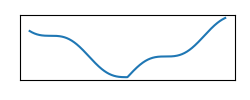
\includegraphics[width=0.3\linewidth]{./ImageFiles/Data Generation/function_example}
	\caption{Generated image example}
	\label{fig:function_example}
\end{figure}
